\section{Adaptivity to \texorpdfstring{$\mu^\star$}{}}\label{app:dttts.adapt}

We now propose a natural extension of \DTTTS to overcome the issue mentioned in the previous section. In this section we assume that we have the knowledge of the maximum mean $\mu^\star$ of the reservoir. The core idea is to keep the same algorithm but with a different prior distribution over each queried arm, that is supported on $[0, \mu^\star]$ instead of $[0, 1]$.

\paragraph{Bernoulli bandits}
We still assume a Bernoulli bandit model for the rewards (although the algorithm is extended to any rewards bounded in $[0,1]$ with the binarization trick): An arbitrary arm produces at time $t$ a reward 1 with probability $\theta$ and a reward 0 with probability $1-\theta$. The likelihood can be written as follow:
\[
    p(s|\theta) = \theta^s(1-\theta)^{1-s}; s\in\{0;1\}.
\]

\paragraph{Sample from the shifted posterior}
In order to implement the extension of \DTTTS, we need to know how to sample from the "shifted" posterior, that is the posterior assuming a uniform prior over $[0,\mu^*]$ instead of $[0,1]$. We now explain how to compute this posterior distribution on $\theta$ given a sequence of observations $Y_1,Y_2,\cdots,Y_N\in\{0;1\}$. Define
\[
    \left\{
    \begin{array}{ll}
        a &= \sum_{i=1}^N Y_i + 1 \\
        b &= N - \sum_{i=1}^N Y_i + 1,
    \end{array}
    \right.
\]
then, according to the Bayes rule, we have
\begin{align*}
    p(\theta|Y_1,\cdots,Y_N) &= \frac{p(Y_1,\cdots,Y_N|\theta)p(\theta)}{p(Y_1,\cdots,Y_N)} \\
                             &= \frac{p(Y_1,\cdots,Y_N|\theta)p(\theta)}{\int_0^1 p(Y_1,\cdots,Y_N|\theta')p(\theta')\1_{[0,\mu^\star]}(\theta')d\theta'} \\
                             &= \frac{\theta^{a-1}(1-\theta)^{b-1}\1_{[0,\mu^\star]}(\theta) / B(a,b)}{\int_{0}^{\mu^\star}(\theta')^{a-1}(1-\theta')^{b-1} / B(a,b) d\theta'} \\
                             &= \frac{\theta^{a-1}(1-\theta)^{b-1}\1_{[0,\mu^\star]}(\theta)}{B(a,b)F_{a,b}(\mu^\star)},
\end{align*}
where $F_{a,b}$ is the \emph{cumulative distribution function} (cdf) of $\texttt{Beta}(a,b)$. Thus the cdf of the posterior is
\[
    \PP{\theta\leq x | Y_1,\cdots,Y_N} = \frac{F_{a,b}(x)}{F_{a,b}(\mu^\star)} \eqdef G(x).
\]
Now the sampling is quite straightforward as $G^{-1}(u)$ can be computed as
\[
    G^{-1}(u) = F_{a,b}^{-1} (u * F_{a,b}(\mu^\star)).
\]
The computation of $F_{a,b}^{-1}$ and $F_{a,b}$ is easily accessible via existing libraries in different programming languages, and we can thus apply \emph{inverse transform sampling} to obtain the observations, since if $U \sim \cU([0,1])$, then $G^{-1}(U)$ follows the posterior distribution.

\paragraph{Shifted Beta distribution}
Recall that we defined a shifted Beta distribution $\texttt{SB}_{\mu^\star}(a,b)$ as the distribution of the random variable $\theta' \eqdef \mu^\star \theta$, where $a, b$ are the shape hyper-parameters of the Beta distribution and $\theta \sim \texttt{Beta}(a,b)$. The \emph{probability density function} (pdf) of $\texttt{SB}_{\mu^\star}(a,b)$ can be written as
\[
    p(\theta') = \frac{1}{B(a,b)} \frac{(\theta')^{a-1}(\mu^\star-\theta')^{b-1}}{(\mu^\star)^{a+b-1}},
\]
via the transformation $\theta' = \mu^\star\theta$. Here $B$ is the Beta function\footnote{$B(a,b)\eqdef\frac{\Gamma(a)\Gamma(b)}{\Gamma(a+b)}$, and $\Gamma$ is the Gamma function}.

The previous expression is particularly useful if we want to use the same efficient implementation trick that we employed in Algorithm~\ref{alg:dttts}, namely the order statistic trick.

\paragraph{Order statistic trick}
Now we show that an "order statistic trick" still exists under a uniform prior over $[0,\mu^*]$, namely that the maximum of $k$ random variables drawn from this prior distribution still has a nice distribution.

Given $n$ random variables $X_1, X_2, \cdots, X_n$, the order statistics $X_{(1)}, X_{(2)}, \cdots, X_{(n)}$ are also random variables, defined by sorting the values of $X_1, X_2, \cdots, X_n$ in an increasing order. In this section we treat the special case where they are i.i.d samples from the same distribution with a cdf. $F_X$.
Following \cite{gentle2009}, Chapter 1 Section 7, we know that the cumulative distribution function of the $k$-th order statistic can be written as follow:
\[
    F_{X_{(k)}}(x) = \sum_{j=k}^{n} (F_X(x))^j (F_X(x))^{n-j}.
\]

%\todo[inline]{Ici on ne s'intéresse qu'à la loi du maximum, ce n'est peut être pas la peine d'écrire l'expression si générale? Au moins dans la formule ci dessous, prend $k=1$}

Now, in our case, where the underlying distribution is the uniform distribution defined over $[0, \mu^\star]$, we obtain the pdf of the order statistic $X_{(k)}$ as follow:
\begin{align*}\label{eq:sb}
\begin{split}
    p_{X_{(k)}}(\theta') &= \frac{n!}{(k-1)!(n-k)!} (\mu^\star)^n (\theta')^{k-1}(\mu^\star-\theta')^{n-k} \\
                        &= \frac{1}{B(k, n+1-k)} \frac{(\theta')^{k-1}(\mu^\star-\theta')^{n-k}}{(\mu^\star)^{(k-1)+(n-k)+1}}.
\end{split}
\end{align*}

We recognize the density of a shifted Beta distribution with $k$ and $n+1-k$ as shape hyper-parameters. In particular, in our case, the pseudo arm at time $t$ is endowed with the distribution $\texttt{SB}_{\mu^\star}(t-k_t,1)$.

\paragraph{Some illustrations of the fix}

Now we show some synthetic results after the previous tricks. Fig.~\ref{fig:shift_fix} shows the expected simple regret of \DTTTS compared to \ISHA, again, under $\texttt{Beta}(0.5,0.5)$, $\texttt{SB}_{0.8}(0.5,0.5)$, $\texttt{SB}_{0.6}(0.5,0.5)$, $\texttt{SB}_{0.4}(0.5,0.5)$ and $\texttt{SB}_{0.2}(0.5,0.5)$ reservoir respectively. We can see that the performance of \DTTTS for shifted cases has been significantly enhanced.

\begin{figure}[ht]
  \centering
  \begin{subfigure}[t]{0.33\textwidth}
    \centering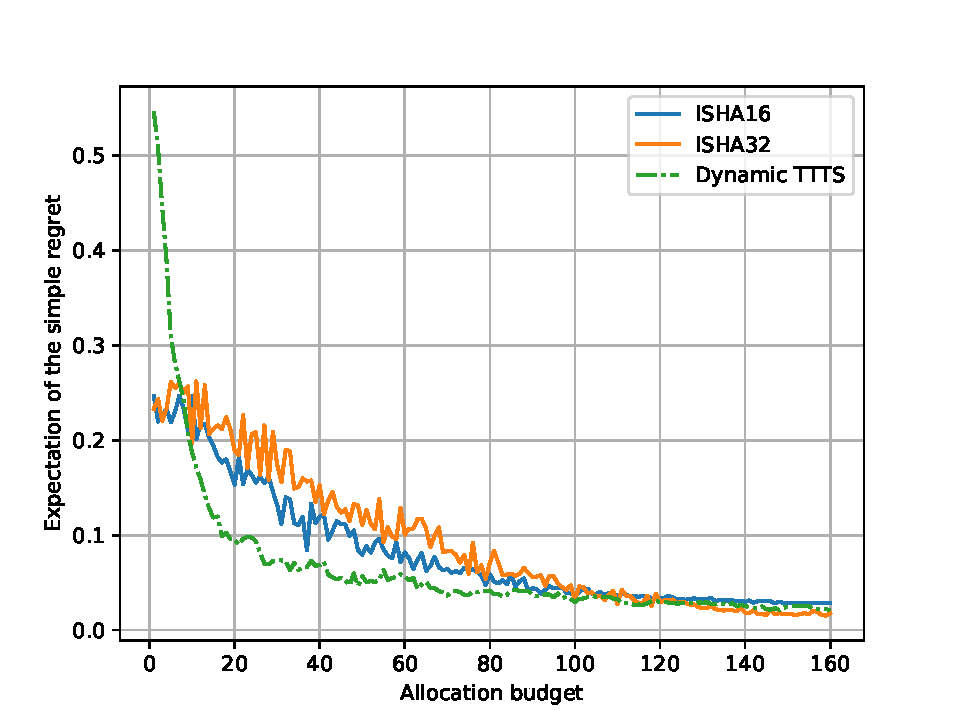
\includegraphics[width=\textwidth]{Chapter6/img/shift/no_shift_fix.pdf}
    \caption{no shift}
  \end{subfigure}%
  \begin{subfigure}[t]{0.33\textwidth}
    \centering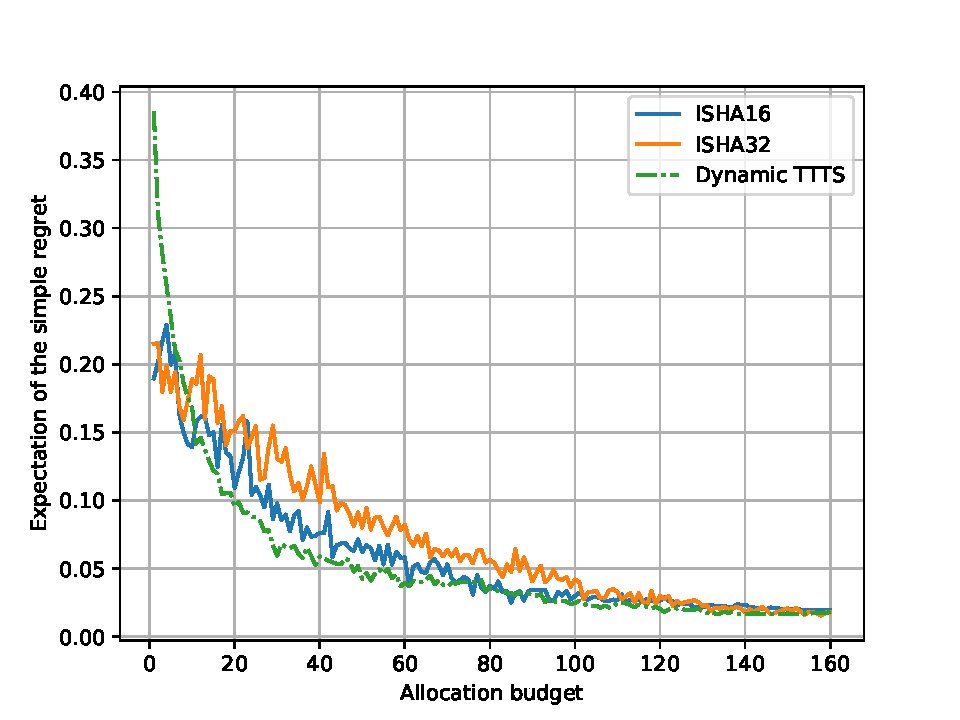
\includegraphics[width=\textwidth]{Chapter6/img/shift/shift_-8_fix.pdf}
    \caption{shift by 0.8}
  \end{subfigure}
    \begin{subfigure}[t]{0.33\textwidth}
    \centering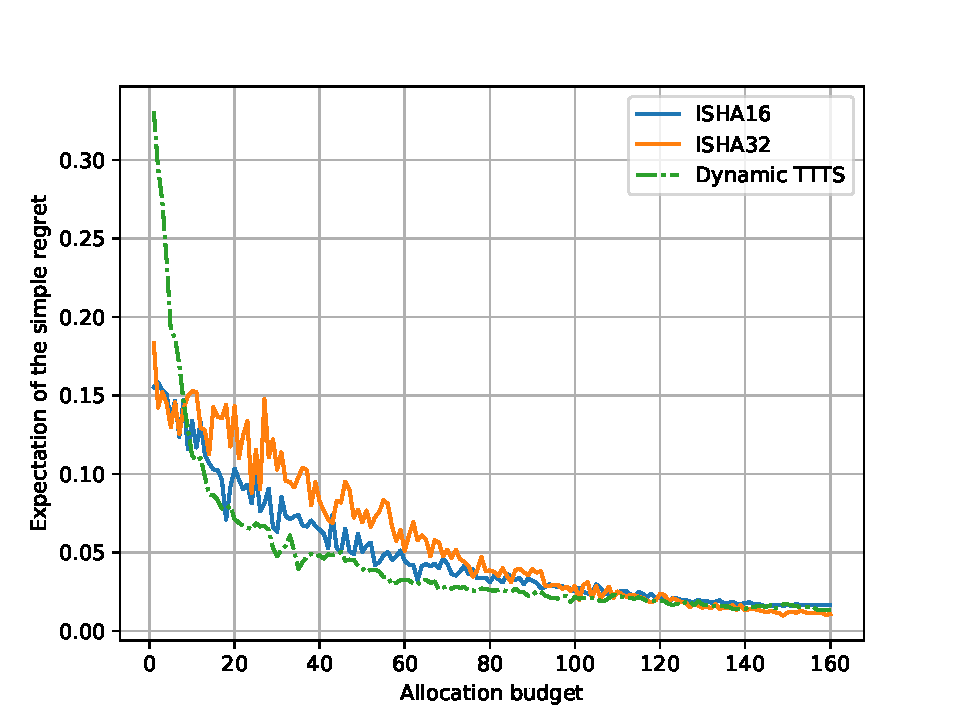
\includegraphics[width=\textwidth]{Chapter6/img/shift/shift_-6_fix.pdf}
    \caption{shift by 0.6}
  \end{subfigure}%
  \begin{subfigure}[t]{0.33\textwidth}
    \centering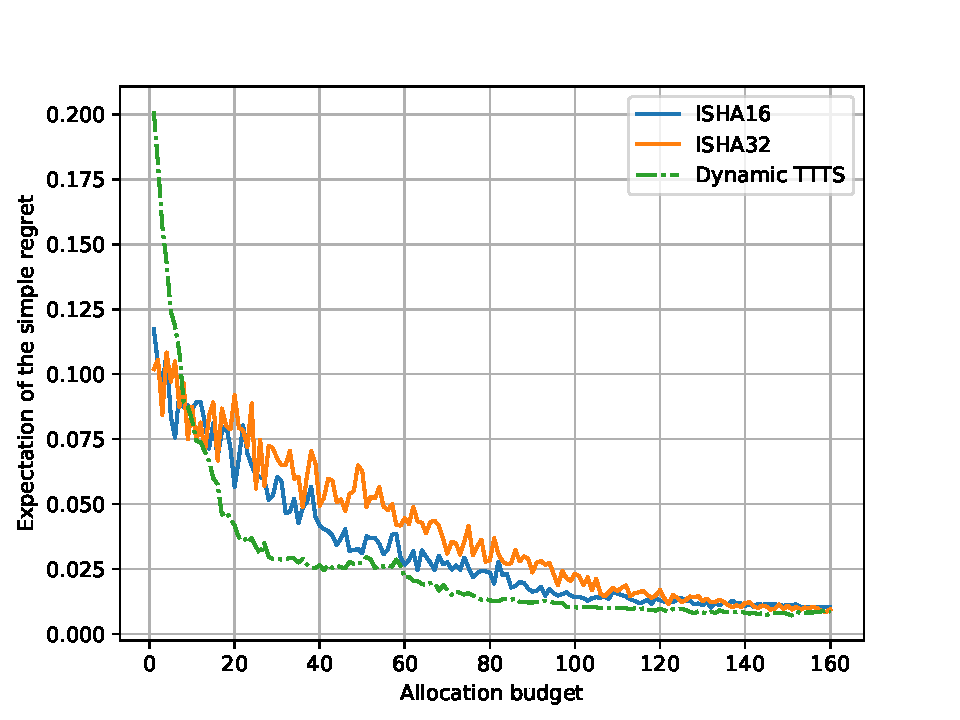
\includegraphics[width=\textwidth]{Chapter6/img/shift/shift_-4_fix.pdf}
    \caption{shift by 0.4}
  \end{subfigure}
  \begin{subfigure}[t]{0.33\textwidth}
    \centering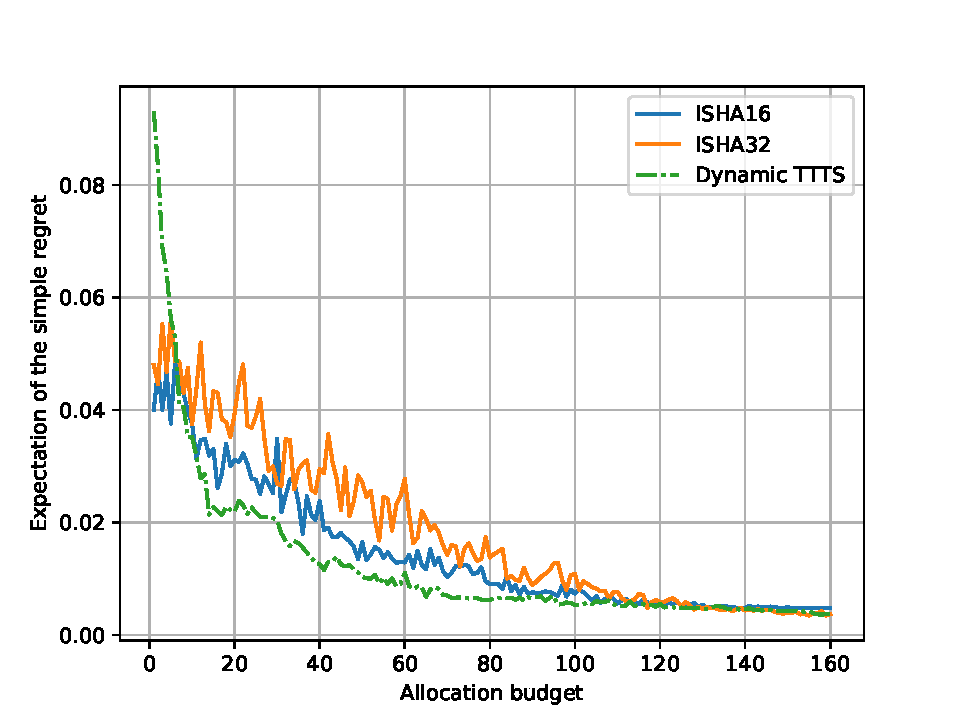
\includegraphics[width=\textwidth]{Chapter6/img/shift/shift_-2_fix.pdf}
    \caption{shift by 0.2}
  \end{subfigure}%
  \caption{Simple regret of \DTTTS for shifted Beta reservoir after the fix.}
  \label{fig:shift_fix}
\end{figure}

We can also compare the number of effectively sampled arms under shifted Beta reservoirs before and after the fix, as shown in Fig.~\ref{fig:arms_fix}. Fig.~\ref{fig:arms_shift_restate} is the same figure as Fig.~\ref{fig:arms_shift}, and Fig.~\ref{fig:arms_shift_fix} is the number of effectively sampled arms after the previous fix under a $\texttt{Beta}(0.5,0.5)$, $\texttt{SB}_{0.8}(0.5,0.5)$, $\texttt{SB}_{0.6}(0.5,0.5)$, $\texttt{SB}_{0.4}(0.5,0.5)$ and $\texttt{SB}_{0.2}(0.5,0.5)$ reservoir respectively. Indeed, we can see that now the exploration effort of \DTTTS under shifted Beta priors is more or less at the same level as that under a normal Beta reservoir. 

\begin{figure}[ht]
  \centering
  \begin{subfigure}[t]{0.45\textwidth}
    \centering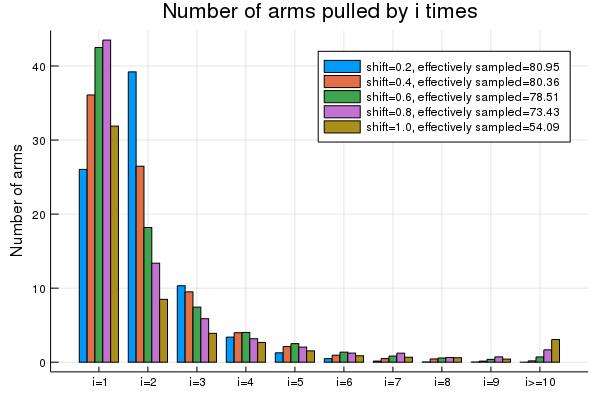
\includegraphics[width=\textwidth]{Chapter6/img/infinite/pulls_shift.png}
    \caption{shift}
    \label{fig:arms_shift_restate}
  \end{subfigure}%
  \begin{subfigure}[t]{0.45\textwidth}
    \centering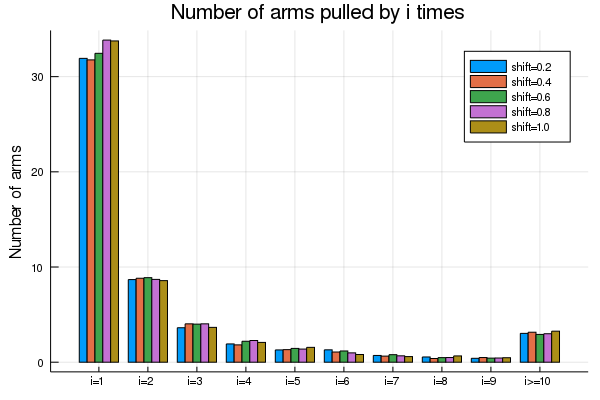
\includegraphics[width=\textwidth]{Chapter6/img/infinite/pulls_shift_fix.png}
    \caption{shift after fix}
    \label{fig:arms_shift_fix}
  \end{subfigure}
  \caption{Distribution of effectively sampled arms of \DTTTS before and after the fix.}
  \label{fig:arms_fix}
\end{figure}
